% Negative-result paper, AAAI-27 workshop W30:
% Effective and Efficient Evaluation for AI Scientists. Anonymised, double-blind.
\documentclass[letterpaper]{article}
\usepackage{aaai2027}
\usepackage{times}
\usepackage{helvet}
\usepackage{courier}
\usepackage[hyphens]{url}
\usepackage{graphicx}
\usepackage{natbib}
\usepackage{caption}
\usepackage{booktabs}
\usepackage{amsmath}
\usepackage{amssymb}
\usepackage{newfloat}
\usepackage{listings}
\urlstyle{rm}
\def\UrlFont{\rm}
\frenchspacing
\setlength{\pdfpagewidth}{8.5in}
\setlength{\pdfpageheight}{11in}

\setcounter{secnumdepth}{2}

\title{Most of It Was Toxicity:\\
A One-Line Control That Invalidates a Phenotype Benchmark}
\author{Anonymous Submission}
\affiliations{}

\begin{document}
\maketitle

\begin{abstract}
An AI scientist is only as trustworthy as the benchmark that scores it, and in the
experimental sciences that benchmark is usually assembled after the fact from
measurements collected for some other purpose. We report three ways this went wrong
in a single case study, a language-conditioned system that retrieves compounds and
doses from a public industrial Cell Painting archive, and the cheap controls that
caught each one. First, the literal reading of per-cell morphology features turned the
benchmark into a cytotoxicity detector: the system scored AUC $0.842/0.873$ on held-out
chemistry while a baseline that never reads the request, obtained by taking the model's
own prediction for \emph{``kill most of the cells''} and using that single vector to
score every other request, scored $0.833/0.855$. The cause is that per-cell features
are averaged over segmented survivors, and dying cells round up and read brighter, so
64--69\% of wells satisfying a per-cell \emph{``brighter''} predicate had also lost
their cells against a 3.5\% base rate. Redefining each predicate to require surviving
cells lowered the headline to $0.799/0.861$ and raised the margin over that baseline
tenfold. Second, a vision-language model used as a blind judge of the same wells, and
validated behaviour by behaviour against the physical measurements, turned out to rank
unseen compounds \emph{below its own} toxicity-only score. Third, the natural
confidence statistic for refusal, the maximum score over the candidate pool, is an
extreme-value statistic that grows with pool size and does not transfer between pools.
None of these was visible in the headline metric, and all three were caught by controls
that cost nothing once a model is trained. We argue that a trivial-baseline control, a
judge-validity table, and a pool-size invariance check should be default reporting for
AI-scientist evaluations, and we release the protocol.
\end{abstract}

\section{Introduction}

Evaluating an AI scientist means evaluating a benchmark first. In silico, the labels
are given. In the experimental sciences they are not: a system that proposes
interventions is scored against measurements that were collected for other reasons,
and the analyst must \emph{define} what counts as success. That definition is a
modelling decision, it is rarely stated as one, and this paper reports a case in which
getting it wrong inflated every number by more than the size of the effect being
claimed, while making the headline metric look better.

The case study is a system that takes an English description of a desired cellular
appearance, for example \emph{``make the mitochondria dimmer without killing the
cells''}, and returns a ranked list of (compound, dose) pairs from a public industrial
Cell Painting archive~\citep{kraus2025rxrx3core}, together with a decision to refuse
when the archive contains nothing suitable. The archive holds 1{,}671 compounds at
eight doses in human endothelial cells, imaged in six fluorescent
channels~\citep{bray2016cellpainting}, summarised by
CellProfiler~\citep{carpenter2006cellprofiler} features.

We report three evaluation failures and the controls that caught them. We report them
because each was invisible in the headline metric, each was caught by a control that is
free once a model exists, and each generalises beyond this archive.

That a model can score well for a reason unrelated to the stated task is not new.
\citet{chuang2018adversarial} argue for adversarial controls in scientific machine
learning, \citet{wallach2018memorization} show that common ligand-based benchmarks
reward memorisation rather than generalisation, and \citet{geirhos2020shortcut} give
the general account of shortcut learning. What we add is specific and, we think,
transferable: the dominant confound of a domain can be turned into a baseline using
the model under test itself, with no extra training and no extra data, simply by
freezing its answer to one request and reusing it for all the others. We also treat
abstention as a scored output rather than as a safety afterthought, which places this
work alongside selective prediction~\citep{geifman2017selective} but at the level of a
request rather than a sample.

\section{Control 1: a baseline that never reads the request}

\subsection{The control}

Given a trained goal-conditioned model, take its prediction for one fixed request,
\emph{``kill most of the cells''}, and use that single vector of scores to rank
candidates for \emph{every other} request. The resulting scorer is blind to the
question. Report it beside every number. The implementation is one line.

A second, equally cheap control ranks by dose alone.

\subsection{What it caught}

Compounds are split by Bemis-Murcko scaffold~\citep{bemis1996scaffold}, so a test
compound shares no ring skeleton with any training compound; numbers are five-seed
ensembles on held-out requests.

\begin{table}[t]
\centering
\small
\begin{tabular}{lcc}
\toprule
\textbf{Literal predicates} & unseen phrasing & unseen concept \\
\midrule
goal-conditioned model      & 0.842 & 0.873 \\
toxicity-only baseline      & 0.833 & 0.855 \\
dose-only baseline          & 0.758 & 0.775 \\
\textit{margin over toxicity} & \textit{+0.010} & \textit{+0.018} \\
\midrule
\textbf{Survival-conditioned predicates} & & \\
\midrule
goal-conditioned model      & 0.799 & 0.861 \\
toxicity-only baseline      & 0.696 & 0.789 \\
dose-only baseline          & 0.722 & 0.761 \\
\textit{margin over toxicity} & \textit{\textbf{+0.104}} & \textit{\textbf{+0.072}} \\
\bottomrule
\end{tabular}
\caption{AUC on compounds whose scaffold the model never saw. Under the literal
predicate definition the system scores higher and sits almost on top of a scorer that
never reads the request. The behaviour-specific contribution is $+0.010$/$+0.018$.
Requiring the cells to survive lowers the headline and multiplies the margin by ten.}
\label{tab:baselines}
\end{table}

Table~\ref{tab:baselines} is the result. Read without the control, the first block is a
respectable phenotype model. Read with it, the first block is a cytotoxicity detector
with a language interface: almost everything it knows, it knows about killing cells.

\subsection{Why the labels did that}

CellProfiler's per-cell features are averages over the objects it can segment, which
are the cells that are still present. A dying cell rounds up and condenses and
therefore reads \emph{brighter} per unit area. The entanglement is directly
measurable. Against a base rate of 3.5\% of (compound, dose) groups showing cell loss,
the share of groups satisfying a per-cell predicate that have also lost their cells is
69\% for brighter DNA, 66\% for brighter actin, 64\% for brighter mitochondria, 62\%
for smaller nuclei, 56\% for fainter actin, 49\% for bigger nuclei, 42\% for dimmer
mitochondria, 37\% for dimmer DNA, and 16\% for elongation (Figure~\ref{fig:confound}).

\begin{figure}[t]
\centering
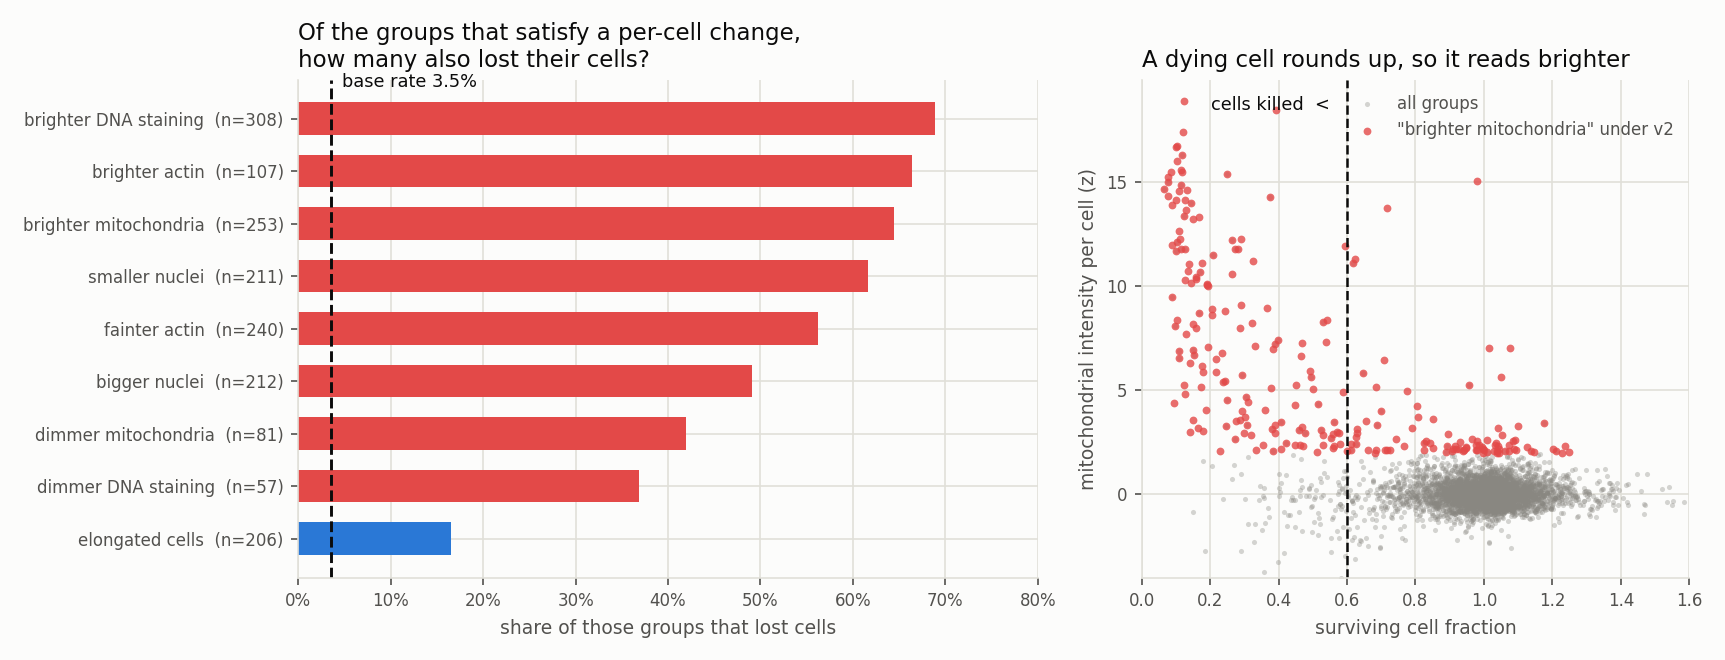
\includegraphics[width=\columnwidth]{figures/03_the_definition_problem.png}
\caption{Left: for each per-cell predicate, the share of satisfying groups that also
lost their cells, against the 3.5\% base rate (dashed). Right: per-cell mitochondrial
intensity against surviving fraction; groups satisfying the literal predicate are
concentrated where the cells are gone.}
\label{fig:confound}
\end{figure}

So \emph{``make the mitochondria brighter''}, read literally off the features, is
substantially a synonym for \emph{``kill the cells''}. A model fitted to that target
learns the shortcut because the shortcut is what the label says. The repair is to
define every per-cell predicate as a conjunction, \emph{$X$ holds in the measured cells
and the cells were not killed}, with the exception of requests that ask for cell loss.
Under the repaired definition the set of requests that nothing in the archive satisfies
grows from 25 to 37, because conjunctions such as \emph{``bigger nuclei and brighter
mitochondria''} occur only in dying cells.

This is not the observation that morphology predicts cell health, which is
established~\citep{way2021cellhealth}. It is that the coupling silently redefines what
a goal-conditioned benchmark measures, while improving its headline number, and that a
free control detects it.

\section{Control 2: validating the judge behaviour by behaviour}

A common design for AI-scientist pipelines replaces the engineered measurement with a
vision-language model acting as a judge. We tested that substitution on the same wells.
Two thousand (compound, dose) groups were rendered as a treated panel beside a
reference panel from the same plate, six channels, native-resolution crops, with one
brightness scale per channel taken from the reference; group identifiers were blind.
The judge returned scores from 0 to 100 with 50 meaning ``no different from the
reference''. Calibration was label-free, so the physical measurements were never used
to fit it, and the calibrated scores then drove exactly the same predicate formulas as
the measurements. Only the instrument differs.

\begin{table}[t]
\centering
\small
\begin{tabular}{lc@{\hskip 1.2em}lc}
\toprule
behaviour & AUC & behaviour & AUC \\
\midrule
cell loss          & 0.93 & brighter mitochondria & 0.69 \\
elongation         & 0.87 & bigger nuclei         & 0.66 \\
dimmer DNA         & 0.81 & brighter DNA          & 0.59 \\
dimmer mitochondria& 0.75 & smaller nuclei        & 0.58 \\
fainter actin      & 0.74 & brighter actin        & 0.73 \\
\bottomrule
\end{tabular}
\caption{Agreement between a blind vision-language judge and the physical measurement,
behaviour by behaviour, over 2{,}000 groups. A single aggregate number would have hidden
the spread.}
\label{tab:judge}
\end{table}

Table~\ref{tab:judge} is the validity table. The pattern is interpretable rather than
random: the judge is reliable at counting and at gross shape, mediocre at ``dimmer'',
and weakest at ``brighter'' and at small size changes, which are exactly the
comparisons a human eye also finds hard across two panels.

The decision-level result is worse than the instrument-level one. \textbf{Trained as a
label source, the judge branch ranks unseen compounds below its own toxicity-only
score} ($-0.02$/$-0.08$ AUC). Doubling the labels from 1{,}000 to 2{,}000 groups gained
$+0.04$ and then saturated; those 2{,}000 groups already cover 100\% of the positives
that exist in the archive for these behaviours, so the ceiling is the archive and not
the annotation budget. A reliability check alone, for instance test-retest agreement,
which was 0.80--0.93 here, would have endorsed the judge. Validity against an
independent measurement, per behaviour, did not.

One further observation is about rendering rather than modelling, and it was the
largest single effect we measured anywhere. In an earlier round each panel was contrast
stretched against its own percentiles before being shown to the judge. The same judge
then scored at chance on four of eight behaviours, because a dim treated well and a
bright reference well rendered identically. A single shared brightness scale moved those
four behaviours to AUC $0.81$--$1.0$. When a judge appears incapable, the presentation
is worth auditing before the model is.

\section{Control 3: is the confidence statistic pool-size invariant?}

A system that always answers cannot be used for screening, so our system abstains when
the archive contains nothing suitable, over 37 requests that no (compound, dose) group
satisfies against 64 that are satisfiable. The obvious confidence statistic is the
maximum predicted score over the candidate pool.

The maximum is an extreme-value statistic and grows with the size of the pool.
Measured here, going from 1{,}256 to 2{,}670 candidate groups, the median maximum for
\emph{unsatisfiable} requests rose from $0.038$ to $0.083$ while the satisfiable ones
did not move. Two consequences follow, and both are evaluation failures rather than
model failures. A threshold calibrated on one pool does not transfer to a larger one.
And a single lucky candidate suffices to answer a request that nothing satisfies.

Replacing the maximum by the mean of the top ten scores, the length of the shortlist
the system displays and therefore fixed in advance, raises refusal AUC from $0.79$ to
$0.85$. A related failure: calibrating the abstention threshold on \emph{training}
compounds, where the model fits closely and its confidence is systematically higher
than it will ever be on new chemistry, produced a threshold that answered only 16\% of
answerable requests; calibrating on validation compounds gave 89\%.

\section{Evaluating in the units of the decision}

AUC states how a ranking is ordered, not what it costs. For a system meant to reduce
experimental work, the decision-relevant question is whether a budget of $k$ wells
contains something that actually does what was asked.

\begin{figure}[t]
\centering
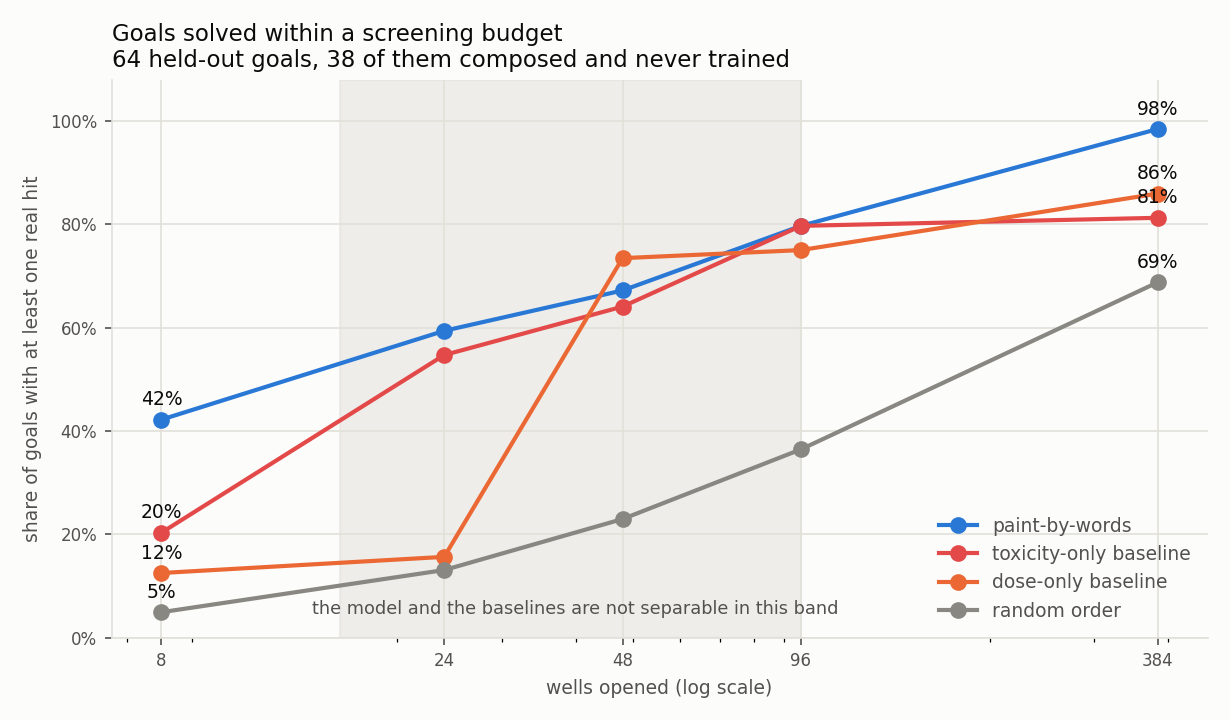
\includegraphics[width=\columnwidth]{figures/06_screening_budget.png}
\caption{Requests satisfied within a budget of $k$ wells, over 64 held-out requests on
unseen chemistry, 38 of them conjunctions whose concept was never trained.}
\label{fig:budget}
\end{figure}

Figure~\ref{fig:budget} reports it, and the honest reading is mixed. Random order needs
a median of 267 wells to reach a first real hit and the system needs 12, which sounds
decisive until the toxicity-only baseline is placed beside it at 18, and until one
notices that at a budget of 48 wells the dose-only baseline beats the system outright
(73\% against 67\%). Goal-specific skill survives in two places: at a budget of eight
wells, one row of a 96-well plate, the system satisfies 42\% of requests against 20\%
for toxicity-only (paired difference $+22\%$, 95\% CI $[+11\%,+33\%]$, 15 requests
satisfied only by the system against 1 only by the baseline, McNemar $p=0.0005$); and at
384 wells, 98\% against 81\%, so roughly one request in five is unreachable along the
toxicity route at any budget. Between 16 and 96 wells nothing is separable.

A single aggregate would have reported either a triumph or a tie depending on where it
was taken.

\section{Recommendations}

From this case study we would make three checks default in AI-scientist evaluation,
each of which is free once a model has been trained.

\paragraph{Report a request-blind baseline beside every number.} Take the model's own
prediction for one fixed, dominant request and score every other request with it. If
the margin is small, the benchmark is measuring the dominant axis and not the stated
task. The dominant axis is domain-specific: cytotoxicity here, and plausibly
solubility, assay interference or sequence length elsewhere.

\paragraph{Validate a judge per behaviour, against an independent instrument.}
Reliability is not validity: our judge was reproducible and still below a trivial
baseline at the decision level. Publish the per-behaviour table, not the mean, and
audit the presentation given to the judge before concluding anything about the judge.

\paragraph{Check that the reported statistic is invariant to the evaluation pool.}
Any extreme-value statistic, maxima and minima above all, is a function of how many
candidates were scored, and thresholds built on it do not transfer.

\section{Limitations}

One archive, one cell type, and 64 held-out requests; the effect sizes in
Figure~\ref{fig:budget} are small and are retrospective, since no prediction here has
been tested at the bench. Compounds are held out by scaffold, but training and test
share plates, so batch transfer is unmeasured: in this archive 1{,}661 of 1{,}671
compounds appear in only one experiment, so holding out an experiment would hold out its
chemistry too and the two effects could not be separated. We state the controls as
necessary, not sufficient: they caught three failures here and say nothing about the
failures they do not test.

\section{Conclusion}

Three evaluation failures in one pipeline, none visible in its headline metric: a label
definition that turned a phenotype benchmark into a toxicity detector while improving
the number, a language-model judge that was reliable and invalid at the same time, and a
confidence statistic that was a function of the pool rather than of the model. Each was
caught by a control costing nothing. We would not have found our own first error without
the request-blind baseline, and we suspect it is worth running wherever a system is
scored on labels derived from measurements that were made for something else.

\section*{Reproducibility}

Code, the full request set with its splits, the exact prompt given to the judge, and
every figure and table in this paper are regenerated by a single command in an
anonymised repository that will be linked in the camera-ready version. Predicate
thresholds were fixed before any training run and never tuned.

\bibliographystyle{aaai2027}
\bibliography{refs}

\end{document}
